\documentclass{article}
\usepackage{amsmath}
\usepackage{amssymb}
\usepackage{graphicx}
\usepackage{hyperref}
\usepackage[version=4]{mhchem}


\begin{document}
In \(\triangle A B C\), point \(E\) is the midpoint of \(A B\). Extend \(A B\) to \(D\) such that \(A B=B D\). Show that \(C D=2 C E\).

Solution:
Draw \(B F / / A C\) to meet \(C D\) at \(F\).\\
Since point \(B\) is the midpoint of \(A D, F\) is the midpoint of \(C D\) and\\
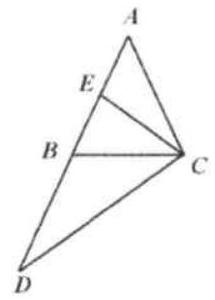
\includegraphics[width=\textwidth]{images/118(1).jpg} \(B F=\frac{1}{2} A C\).

Since point \(E\) is the midpoint of \(A B, B E=A E\)\\
\(\frac{1}{2} A B=\frac{1}{2} A C=B F\).\\
\centering
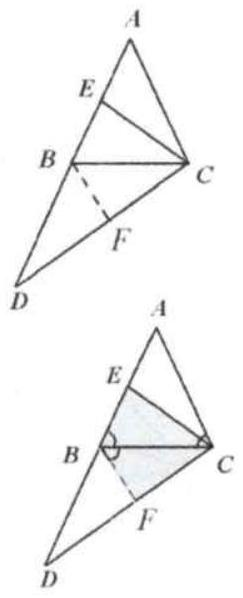
\includegraphics[width=\textwidth]{images/118(2).jpg}

Since \(B F / / A C, \quad \angle F B C=\angle B C A=\angle C B A . B C=B C\).\\
Thus \(\triangle F B C \cong \triangle E B C\).\\
Thus \(C E=F C=\frac{1}{2} C D \quad \Rightarrow \quad C D=2 C E\).


\end{document}
